\chapter{Experimental Evaluation}

\noindent For the purposes of evaluating Modulo7, test cases have been designed into two formats. One category of testing is micro testing, for validating correctness and precision recall for small sets of data. This ensures verifiability of algorithms and similarity measures on small datasets as well as novel explorations of data. Most MIR research is done on small scale datasets and hence falls in the purview of micro testing. The other format is macro testing which involves large datasets such as the million song dataset \cite{msd}. \\\\
A few assumptions that are made in testing are as follows :-
\begin{enumerate}
% TOD0 : Finish this section
\item In order to estimate ground truth values, the author assumed ground truth values presented in datasets used / or subjective judgements to which songs are similar to each other. These subjective judgements are procured from existing literature.
\item If the song metadata (such as keysignature, timesignature, total duration of song) is not encoded, its estimated by the parsers. This estimation id done by existing algorithms in literature. However if metadata is encoded, its assumed to be correct. 
\item Most tests are against file formats of the similar types (for example midi is tested against other symbolic files). This is due to the inherent complexity of symbolic decoding of audio formats like mp3. Also its easier to compare symbolic data against other symbolic data.
\item In the event of parsing data, there can be legal issues (e.g. the song can be copyrighted). For that reason custom parsers to build alternate research datasets (e.g the million song dataset has already derived features that Modulo7 intended to derive for Mp3 files. \cite{msd})
\item All evaluations are done against research datasets which are published in academia or exposed as public datasets in industry. 
\end{enumerate}

\section{Results of Index Compression}

\noindent The Modulo7 representation can be thought of an indexed meta data version of the song. True to all indexed data, Modulo7 represents the song in a much smaller size than the original source. The following chart demonstrates the average compression of indexed data as compared to source files on the Saarland Music Data (SMD) Dataset \cite{saarlandmsd}:-
\begin{figure}
\centering
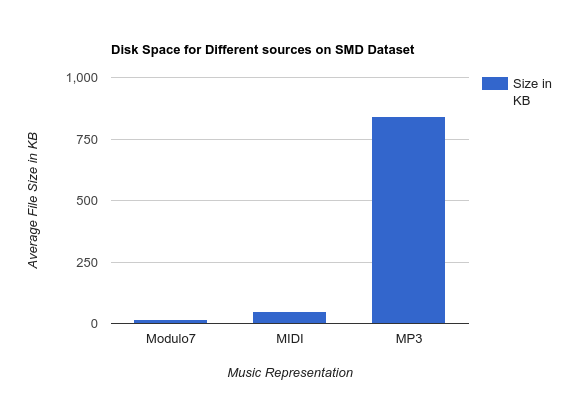
\includegraphics[width=\textwidth]{Modulo7SMDBarGraph.png}
\makeatletter
\let\@currsize\normalsize
\caption{Modulo7 architectural design}
\label{fig:figure}
\end{figure}
As expected Modulo7's serialized format expresses a song in less disk space than its source formats while keeping the symbolic information intact. The results are positive as there is a 4 time decrease in size of expressing symbolic information as compared to midi files. \\\\
A similar transformation was also done on a direct downloadable subset of the wikifonia dataset in order to compare Modulo7 internal representation against normal 

\section{Result on Memory and Disk space \\ usage}

\noindent In order to compare the memory and disk space requirements, Modulo7 was tested against its closest competitor jMIR's \cite{jMIR} jSymbolic component. Both frameworks are written in Java and both involve extraction of features. However jMIR is more exhaustive in what features it extracts so only a subset of those that are also extracted by Modulo7 are considered. 

\section{Results on similarity measures}

\noindent This set of experiments determine the precision and recall values for the similarities defined in \ref{similarity} on ground truth data extracted from \cite{msd}. Modulo7 does not claim to improve on the state of the art when it comes to similarity metrics. However the following tests are carried out : 

\begin{enumerate}
\item Benchmarks are done against the SIMILIE software stack \cite{similie} after taking into account the inherent speed difference between R\cite{similietechnicalmanual} and Java
\item The state of the art similarity measures for melodies are generalized to polyphonic music and tested against newer datasets as compared to \cite{keylist}
\end{enumerate}  

\section{Results on lyrics similarity and statistics analysis}

\noindent On top of the experiments done for Song sources incorporating tonal information, there were specific experiments that were carried out for 